\chapter{Introducción a Matlab}
\section{Introducción}
\textbf{MATLAB} (\textbf{MAT}rix \textbf{LAB}oratory) es un entorno y lenguaje de programación. Su ventaja es su capacidad para realizar operaciones de arreglos multidimensionales como vectores ($n \times 1$), matrices ($n \times m$), etc. de manera rápida y sencilla. \\

\noindent MATLAB tiene documentación para todas sus funciones. Dentro del mismo entorno se puede consultar cómo utilizar una función escribiendo \emph{help nombre\_función} en la ventana de comandos o consultando su página web, la cual contiene ejemplos:

\section{Crear Variables}
Las variables se utilizan para almacenar datos. Hay diversas estructuras de datos para almacenarlos, como escalares, vectores, matrices, también, cadenas de texto (string), celdas (cells), estructuras (struct) a las que se les asignan letras o variables:

\subsection{Crear arreglos}
Un arreglo es un escalar, vector, matriz, etc. Con dimensiones $m \times n \times o \times p \times ...$ \\

Ej: Crear las siguientes variables: $a = 1$, $b = \begin{bmatrix}
1 \\
2 \\
3
\end{bmatrix}
$ y $c = \begin{bmatrix}
1 & 2 & 3 \\
4 & 5 & 6 \\
7 & 8 & 9
\end{bmatrix}
$

\begin{verbatimg}
    a = 1;                          % número escalar (o arreglo de 1 dimensión)
    b = [1; 2; 3];                  % vector de números (o arreglo 3x1)
    c = [1 2 3; 4 5 6; 7 8 9];      % matriz de números (o arreglo 3x3)
\end{verbatimg}

\noindent Los comentarios van con signo de porcentaje \%. Para no mostrar la asignación de la variable en la ventana de comandos, escribir ; al final de la asignación.

\subsubsection{Inicializar arreglos}
Es una buena practica primero inicializar un vector/matriz vacío (llenos de ceros o unos) ya que MATLAB primero asigna un espacio en la memoria, por lo que si se desea añadir un nuevo elemento al arreglo, se tendría que reasignar el espacio en la memoria todas las veces que se modifica.
\begin{verbatimg}
    A = zeros(3,4); % Inicializar matriz con ceros, 3 filas y 4 columnas
    v = zeros(3,1); % Inicializar vector con ceros, 3 filas
    A = ones(5,5);  % Inicializar vector con unos, 5 filas y 5 columnas
\end{verbatimg}

\subsubsection{Vectores desde rango}
Ej: Vector de tiempos para una simulación:
\begin{verbatimg}
    t_inicio = 0; % s
    t_final = 10; % s
    paso_tiempo = 0.1; % s
    t = (t_inicio:paso_tiempo:t_final); % vector fila
\end{verbatimg}

\subsubsection{Recorrer arreglos}
\noindent Para observar qué contiene un arreglo (vector o matriz) en una posición específica:

\begin{itemize}
    \item \emph{matriz(i, j)} para ver el elemento en fila i, columna j
    \item \emph{matriz(i, :)}  para ver la fila i (todas las columnas), vector fila
    \item \emph{matriz(:, j)}  para ver columna j (todas las filas), vector columna
    \item \emph{matriz(:, :)}  toda la matriz
    \item \emph{matriz(i:e, j:k)} para ver matriz entre las filas i y e y las columnas j y k
    \item \emph{vector(j: end)} para ver elemetos en vector desde la fila j en adelante.
    \item \emph{arreglo(i, j, k)} para ver la matriz k en la fila i columna j (se puede ver como un vector de matrices)
\end{itemize}

\subsubsection{Filtrar arreglos}
\begin{verbatimg}
    vector = [1; 0; 2; 0; 3; 4; 0; 5; 0];
    filtro_1 = vector(vector != 0) % tomar todo lo que no es 0, esto retorna filtro_1 = [1; 2; 3; 4; 5]
    filtro_2 = vector(vector == 1) % toma todo lo que es 1, esto es [1]
\end{verbatimg}

\subsubsection{Eliminar elementos}
\begin{verbatimg}
    v(5) = [ ];     % Borrar quinto elemento de un vector
    M(5, :) = [ ];  % Borrar la quinta fila de una matriz
\end{verbatimg}

\subsection{Números complejos}
\begin{verbatimg}
    num_complejo = 1 + 3i;  % crear numero complejo
    real(num_complejo)      % parte real del NC, retorna 1
    imag(num_complejo)      % parte imaginaria del NC, retorna 3
\end{verbatimg}

\subsection{Variables simbólicas}
Si se desea trabajar con expresiones algebraicas se pueden crear \emph{variables simbólicas}. No es recomendable trabajar con variables simbólicas ya que MATLAB es ineficiente para trabajar con este tipo de variables:

\begin{verbatimg}
    syms t          % crear variable 't' (t es una variable tipo simbólica)
    x = 1 + 3*t;    % x es una variable tipo simbólica
\end{verbatimg}

\subsection{Serie de caracteres}
Las series de caracteres se dividen en \emph{strings} y \emph{chars}, cada una tiene sus propias funciones para operar con ellas:
\begin{verbatimg}
    caracteres = 'abcdfghijk';      % char
    caracteres_2 = "qwertyuiop";    % string
\end{verbatimg}

\subsection{Structs}
Para almacenar diferentes tipos de datos en una misma variable, se puede utilizar un \emph{struct} (similar a diccionarios en python):\\

Ej: Para 10 registros sísmicos, guardar los vectores de aceleración del registro, tiempo del registro, aceleración espectral, periodos de la aceleración espectral, duración del registro. 
\begin{verbatimg}
    n_registros = 10;
    dataRegistros = struct()                % inicializar un struct    
    for i =  1:n_registros                  % para cada registro...
        [reg, t] = importReg(registro(i));  % Suponga tenemos función para importar registros
        % Guardar datos en struct
        dataRegistros(i).registro = reg;
        dataRegistros(i).tiempo = t;
        dataRegistros(i).Sa = computeSa(reg, t, T, xi);
        dataRegistros(i).duracion = max(t); % o t(end)
    end
    %  Entonces, para consultar sobre el tiempo del tercer registro
    vector_tiempo_3er_registro = dataRegistro(3).tiempo;
\end{verbatimg}

\noindent Los \emph{structs} organizan y estructuran datos de manera coherente en el código y se utilizan especialmente para simplificar las funciones al reducir la cantidad de inputs necesarios. En lugar de escribir múltiples inputs, se utiliza solo uno que luego se descompone dentro de la función.

\section{Operaciones}
Para saber que tipo de variable es una variable, comando \emph{class()}
\begin{verbatimg}
    A = [1;2;3];
    class(A)  % retorna 'A is double'
\end{verbatimg}

\subsection{Operaciones Básicas}
Las operaciones funcionan igual que las operaciones matriciales y vectoriales. \\

Sumar arreglos (matlab suma componentes (i,j) de cada arreglo)
\begin{verbatimg}
    suma_matrices = matriz_1 + matriz_2;
\end{verbatimg}

Sumar elementos del arreglo
\begin{verbatimg}
    suma_vector = sum(vector_1)
\end{verbatimg}

Restar (matlab resta componentes (i,j) de cada arreglo)
\begin{verbatimg}
    resta_matrices = matriz_1 - matriz_2;
\end{verbatimg}

Multiplicar
\begin{verbatimg}
    matriz_por_matriz = matriz_1*matriz_2;
    vector_por_vector_componente = vector_1.*vector_2;
\end{verbatimg}

Invertir matrices $matriz^{-1}$
\begin{verbatimg}
    matriz_invertida = matriz_1^-1; % o inv(matriz)
\end{verbatimg}

Trasponer matrices $matriz^T$
\begin{verbatimg}
    matriz_traspuesta = matriz_1.';
\end{verbatimg}

Diferenciar e integrar
\begin{verbatimg}
    vector_diferenciado = diff(vector_1);
\end{verbatimg} 

Suma acumulada
\begin{verbatimg}
    vector_suma_acumulada = cumsum(vector_1);
\end{verbatimg}

\noindent Además, MATLAB también incluye las funciones de operaciones matemáticas básicas
\begin{itemize}
    \item log() y exp() - Logaritmo natural y exponencial
    \item sqrt() y ()\^x - Raíces y Potencias
    \item sin() y cos() - Seno y coseno
    \item $X = A\setminus B$ - Solución de $A*X = B$
    \item $X = B/A$ - Solución de $X*A = B$
    \item diag() - de vector a matriz diagonal o extraer diagonal de una matriz
\end{itemize}

\subsection{Función por partes}
Para crear una función por partes se utiliza la función \emph{piecewise()}.

\begin{verbatimg}
    func_por_partes = piecewise(condicion_1, valor_1, condicion_2, valor_2, ...);
\end{verbatimg}

\subsection{Problema de vectores y valores propios}
MATLAB cuenta con la función \emph{eig()} para resolver el problema de vectores y valores propios generalizado.

\begin{verbatimg}
    [vectores_propios, valores_propios] = eig(A, B)
\end{verbatimg}

\noindent $vectores\_propios$ es una matriz donde cada columna es un vector propio y $valores\_propios$ es un vector donde cada elemento es un valor propio.

\subsection{Funciones estadísticas}
Media $\mu$
\begin{verbatimg}
    media = mean(datos_x)
\end{verbatimg}

Desviación estandar $\sigma$
\begin{verbatimg}
    desv_est = std(datos_x)
\end{verbatimg}

Varianza
\begin{verbatimg}
    varianza = var(datos_x)
\end{verbatimg}

Otros
\begin{verbatimg}
    % Autocorrelación
    autocorr_xy = xcorr(datos_x, datos_y) % cross correlation
    % Autocovarianza
    autocov_xy = xcov(datos_x, datos_y) % cross covariance
    % Coeficiente de correlación
    coefic_correl = coff_corr(datos_x, datos_y)
\end{verbatimg}

\subsection{Realizaciones de Variables Aleatorias}
Dependiendo de la distribución se pueden crear realizaciones de variables aleatorias: \\

Ej: 1000 realizaciones de distribución normal estándar $X \sim N(0,1)$
\begin{verbatimg}
    realizaciones = randn(1000,1); % vector (1000 x 1)
\end{verbatimg}

Ej: 1000 realizaciones de la masa de personas si $M \sim N(79.91, 14.89)$
\begin{verbatimg}
    mu = 79.91;                 % media
    sigma = 14.89;              % desviación estándar
    n_realizaciones  = 1000;    % cantidad de realizaciones
    realizaciones_masas = normrnd(mu, sigma, n_realizaciones, 1); 
\end{verbatimg}

Ej: Realizaciones de la siguiente medida de intensidad de registro sísmico: $IM = Sa(T=1[sec], xi = 5\%)$, donde $IM \sim lognormal(0.2, 0.57)$
\begin{verbatimg}
    mu_ln = 0.2;            % g, desde GMPE
    sigma_ln = 0.57;        % g, desde GMPE
    n_realizaciones  = 1000;
    
    realizaciones_IM = exp(mu_ln + sigma_ln*randn(n_realizaciones, 1));
    % desde la media moverse sigma_ln*numero_aleatorio_normal_estandar veces
\end{verbatimg}

\section{Ciclos, iteraciones y condicionales}
Los ciclos (loops) permiten repetir un mismo algoritmo. A pesar de que uno tienda a realizar todo con ciclos, operar vectores y matrices de forma inteligente es más eficiente.

\subsection{Ciclo for}
El ciclo for sirve para repetir el mismo procedimiento un número determinado de veces. \\

Ej: Suponga que tenemos las matrices de la EDM en coordenadas modales $Mn$, $Cn$, $Kn$, el vector con las frecuencias de vibrar de cada modo $wn$. Obtener la fracción de amortiguamiento modal.
\begin{verbatimg}
    xi_n = zeros(5,1) % vector vacío para pre asignar la memoria en tamaño correspondiente
    for n = 1:5 % 5 modos, n es el número del modo
        xi_n(n) = Cn(n,n)/(2*Mn(n,n)*wn(n))
    end
    % Nota, vectorialmente: xi_n = diag(Cn)./(2*diag(Mn).*wn)
\end{verbatimg}

\subsection{Ciclo while}
Repetir el mismo procedimiento hasta que se cumpla una condición. \\

Ej: Contar hasta 100 y mostrar números en pantalla
\begin{verbatimg}
    contador = 0;
    while contador < 100
        fprintf('El contador es: \%.0f \n', contador) 
        contador = contador + 1; % Aumentar el valor del contador
    end
\end{verbatimg}

\newpage
Ej: Encontrar carga última cuando se alcanza una deformación crítica  de 20[cm] utilizando una carga monotónica y un modelo bilineal del material.

\begin{verbatimg}
    % Inputs
    delta_cr = 200;, delta_y = 50; % mm, deformaciones critica y fluencia
    deltas = (0:0.1:400).'; % mm, vector de deformaciones
    k1 = 200; % kN/mm rigidez primer tramo
    alfa = 0.2; % factor de reducción de rigidez para segundo tramo
    % Previo
    k = zeros(length(deltas), 1);
    k(deltas <= delta_y) = k1;, % tramo 1 modelo bilineal
    k(deltas > delta_y) = alfa*k1; % tramo 2 modelo bilineal
    P_y = k1*delta_y; % Carga de fluencia    
    P = zeros(length(deltas),1);, i = 1;, delta_actual = 0;
    % Ciclo while
    while delta_actual <= delta_cr % Repetir siclo hasta cumplir condición
        k_actual = k(i);
        if delta_actual < delta_y % tramo 1
            P_actual = k_actual*delta_actual;
        elseif delta_actual >= delta_y % tramo 2
            P_actual = P_y + k_actual*(delta_actual - delta_y);
        end
        P(i) = P_actual;            % guardar carga en vector
        i = i + 1;                  % para siguiente iteración
        delta_actual = deltas(i);   % para siguiente iteración
    end
    P_simu = P(1:i);                % cargas simuladas
    deltas_simu = deltas(1:i);      % deformaciones simuladas
    P_cr = P_simu(end);             % carga crítica
\end{verbatimg}

\subsection{Condicionales}
Una declaración condicional permite decidir si ejecutar un algoritmo o no si es que se cumple con una condición (cuando booleano es True). \\

Ej: Verificar si una sección cumple con diseño a flexión
\begin{verbatimg}
    phiMn = 20;     % tonf-m Momento flector nominal de la sección reducido.
    Mu = 18;        % tonf-m Momento último que actúa en la sección.
    
    % Condicional
    if phiMn > Mu  
        disp('cumple')
    else
        disp('no cumple')
    end
\end{verbatimg}

Ej: Calcular el factor de longitud efectiva de la zona de compresión del hormigón $\beta_1$ de la norma ACI318, utilizando condicional "if":
\begin{verbatimg}
    fc = 30; % MPa, resistencia hormigón fc = 300 kgf/cm^2
    if fc >= 17 && fc <= 28 % probar con primer rango
        beta1 = 0.85;
    elseif fc > 28 && fc < 55 % si no está en primer rango, probar con segundo rango
        beta1 = 0.85 - (0.05/7)*(fc - 28);
    else % si no está en ninguno
        beta1 = 0.65;
    end
\end{verbatimg}

\section{Funciones}
Las funciones en MATLAB toman variables input, trabajan con ellas y retornan variables output. Las funciones son fundamentales para organizar los scripts (para no escribir lo mismo muchas veces), lo que facilita su comprensión. \\

\noindent Las funciones se pueden crear ya sea en archivos \emph{.m} separados del script general o escribiéndolas al final del código. Si se crean en archivos, el nombre del archivo debe ser el mismo nombre de la función. \\

Ej: Crear una función para calcular $Sa_{avg}$ de un registro sísmico (una medida de intensidad):
\begin{verbatimg}
    function [Sa_avg] = computeSaAvg(Sa, T_vect, T, c1, c2, dT)
        % Interpolación
        T_interp = (c1*T:dT:c2*T).';
        Sa_interp = interp1(T_vect, Sa, T_interp, 'linear', 'extrap');
        
        % Calcular Sa_avg (aplicar log() a ecuación de Eads et al 2015)
        Sa_avg = exp(1/length(Sa_interp)*sum(log(Sa_interp)));
    end
\end{verbatimg}

\noindent El archivo que contiene la función debe guardarse con el mismo nombre de la función, en este caso el nombre del archivo debería ser \emph{computeSaAvg.m}. \\

\noindent Luego, para llamar la función desde el script de matlab, se debe escribir el mismo nombre y los inputs.

\begin{verbatimg}
    % Suponga que ya se obtuvieron Sa y sus periodos respectivos T_vect de un registro sísmico
    T = 1;      % s, Periodo de estudio
    dT = ;      % s, Espaciamiento deseado para la interpolación de T_vect
    c1 = 0.2;   % Para T_min para calcular Sa_avg
    c2 = 3;     % para T_max para calcular Sa_avg

    % Llamar a la función y guardar resultado en una variable
    Sa_avg = computeSaAvg(Sa, T_vect, T, c1, c2, dT)
\end{verbatimg}

\newpage
\section{Importar y exportar datos}
\subsection{Importar}
Matlab permite importar datos desde una gran variedad de archivos (.txt, .csv, .xlsx, ...). Dependiendo del formato en el que estén los datos en los archivos existen diversas funciones. Las más importantes son las siguientes:

\begin{itemize}
    \item readmatrix()  - genera una matriz
    \item readtable()   - genera una tabla
    \item load()        - carga datos
\end{itemize}

\subsection{Exportar}
Para exportar datos también existen funciones:
\begin{itemize}
    \item writematrix()
    \item writetable() 
\end{itemize}

\noindent Revisar la documentación de matlab para entender cómo utilizar las funciones.

\section{Figuras}
Para graficar en matlab se ocupan series de datos como vectores o matrices:

\subsection{Plot}
Ej: Tomando los resultados del pushover de 4.2, graficar la curva de carga vs desplazamiento
\begin{verbatimg}
    % P_simu: vector de cargas simuladas
    % deltas_simu = vector de deformaciones simuladas
    
    figure  % Crea una nueva ventana/figura
    plot(deltas_simu, P_simu,'linewidth',2,'color','r')
    hold on                 % para poner más que un gráfico en la figura
    xline(delta_cr)         % Incluir línea vertical
    yline(P_cr)             % Incluir linea horizontal
    hold off                % para dejar de incluir graficos a la figura
    xlim([0 deltas(end)])   % limitar ancho de ventana
    grid on                 % encender grilla
    xlabel('deformación \delta [mm]')
    ylabel('Carga P [kN]')
\end{verbatimg}

\begin{figure}[H]
    \centering
    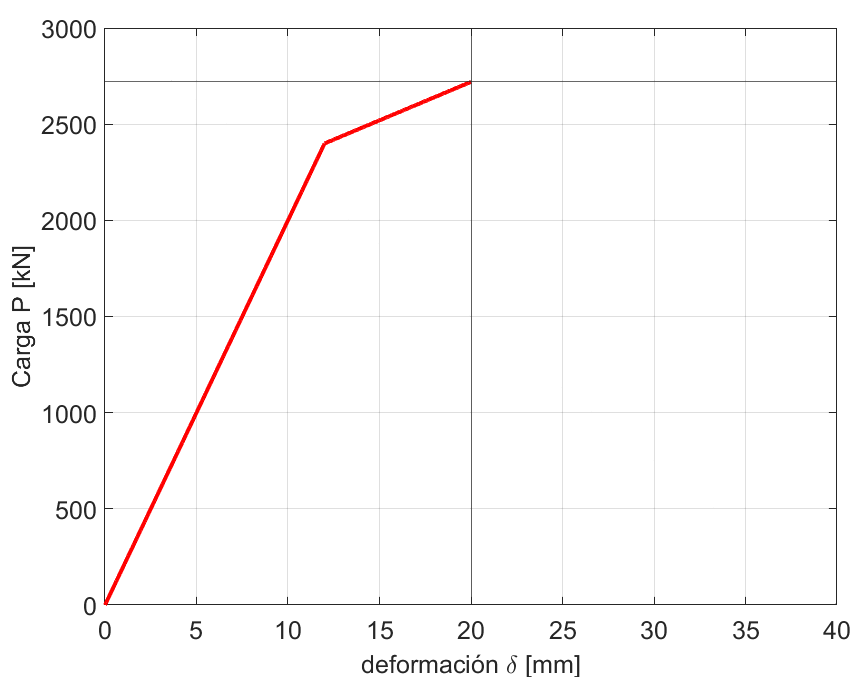
\includegraphics[width=0.55\linewidth]{Figuras/curvCapacidad.png}
\end{figure}

\noindent En la figura, haciendo click en file > export setup, se puede configurar la vista de la figura para exportar.

\subsection{Dispersión}
\begin{verbatimg}
    figure
    scatter(data_x, data_y)
\end{verbatimg}

\subsection{Histogramas}
\begin{verbatimg}
    figure
    histogram(vector_data)
\end{verbatimg}

\noindent También se pueden normalizar los histogramas y hacer ajustes a distribuciones

\begin{verbatimg}
    mu = 79.91;
    sigma = 14.89;
    cantidad_realizaciones = 1000;
    realizaciones_masas = normrnd(mu, sigma, cantidad_realizaciones, 1);

    % Histograma normalizado a pdf
    figure
    histogram(realizaciones_masas, 'normalization', 'pdf')

    % Histograma con ajuste de distribución
    figure
    histfit(realizaciones_masas, 20, 'normal')
    
\end{verbatimg}

\newpage
\noindent El resultado de aplicar \emph{histfit()} con las 1000 realizaciones (simulaciones) de la distribución normal.
\begin{figure}[H]
    \centering
    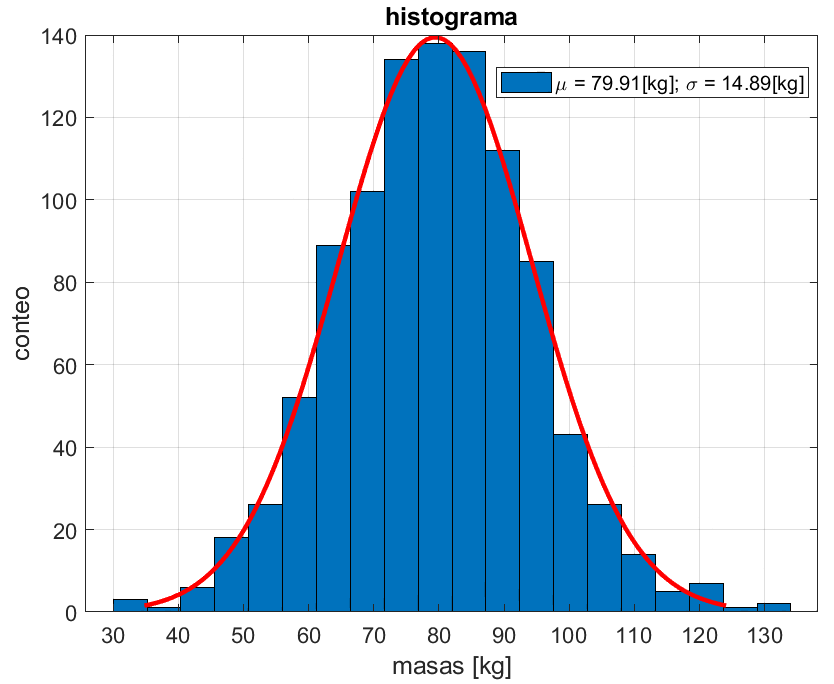
\includegraphics[width=0.55\linewidth]{Figuras/histogramFitting.png}
\end{figure}

\section{Instalar Toolbox}
Para instalar un toolbox, dentro de MATLAB ir a Home > Add-Ons > Get Add-Ons, lo que abrirá una pestaña para buscar e instalar toolbox.

\begin{figure}[H]
  \centering
  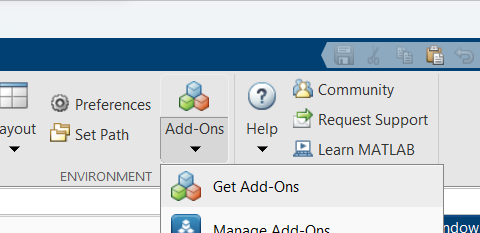
\includegraphics[width=0.47\textwidth]{Figuras/AddOnsButton.png} 
\end{figure}

Un toolbox necesario para el curso es el \emph{Control System}. Instalarlo.
\begin{figure}[H]
    \centering
    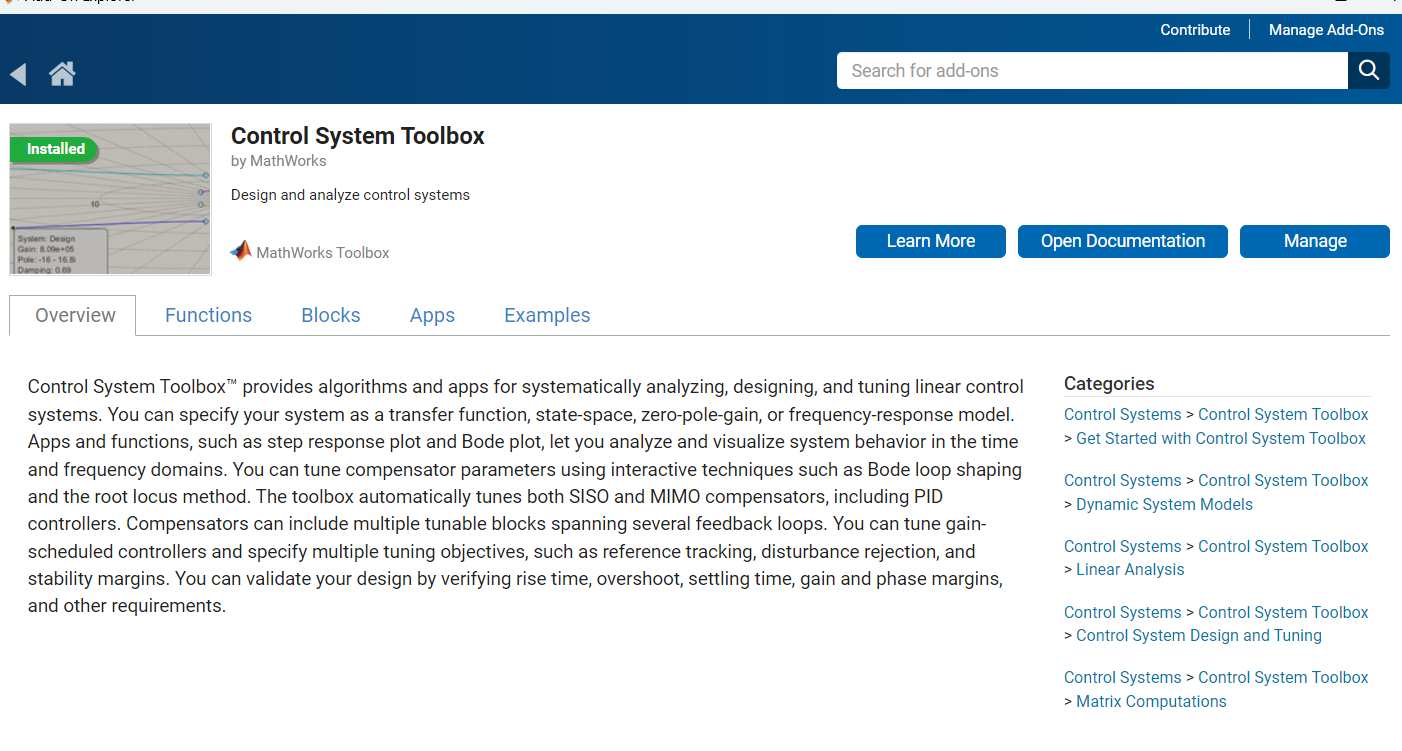
\includegraphics[width=0.75\linewidth]{Figuras/controlSystemToolbox.png}
\end{figure}

\section{Funciones útiles para el curso}
Muchos de los conceptos que se aprenden en cátedra, pueden realizarse en MATLAB con una función. \\

\subsection{Representación de sistemas}
Para trabajar con sistemas en MATLAB, existen las \emph{Variables tipo sistema} que pueden ser creadas con alguna de las repreentaciones vistas en clases (y más). \\

Espacio-Estado (State-Space, SS)
\begin{verbatimg}
    % Ass, Bss, Css, Dss son las matrices de la representación espacio-estado de un sistema
    sys_ss = ss(Ass, Bss, Css, Dss)
\end{verbatimg}

Función de Transferencia (Transfer Function, TF)
\begin{verbatimg}
    % num: vector con los coeficientes del polinomio del numerador de la TF
    % den: vector con los coeficientes del polinomio del denominador de la TF
    sys_tf = tf(num, den);
\end{verbatimg}

Desde State-Space a Transfer Function y viceversa
\begin{verbatimg}
    sys = ss(sys_tf);       % desde sistema en representación TF a SS
    sys = tf(sys_ss);       % desde sistema en representación SS a TF
    sys = ss2tf(A,B,C,D)    % tf desde matrices ss
    sys = tf2ss(num, den)   % ss desde coeficientes tf
\end{verbatimg}

\noindent Da exactamente el mismo sistema si se utiliza la representación state-space o transfer function.

\subsection{Excitar sistemas}
\begin{itemize}
    \item \emph{impulse(sys)}: aplicar impulso al sistema
    \item \emph{ramp(sys)}: aplicar excitación de rampa al sistema
    \item \emph{step(sys)}: aplicar excitación de escalón al sistema
\end{itemize}

\subsection{Otras funciones útiles para el curso}
\begin{itemize}
    \item \emph{damp()} - Polos, frecuencia, amortiguamiento
    \item \emph{bode(), bodeplot()} - Bode
    \item \emph{rootlocus()} - Root-locus
    \item \emph{pzmap()} - Mapa de polos y ceros
    \item \emph{fft(), shiftfft()} - Fast Fourier Transform
    \item \emph{ode45()} - Integración numérica Runge-Kutta Ode4
    \item \emph{expm()}
    \item \emph{repmat()}
\end{itemize}

\noindent Revisar la documentación de estas funciones
